% =====================================================================
%  Technical Report — NLP Search Agent
%  Compile with:  pdflatex TECHNICAL_REPORT.tex   (run twice for refs)
%  Requires a standard TeX Live / MiKTeX install (booktabs, pgfplots,
%  listings, hyperref, geometry — all in the base distribution).
% =====================================================================
\documentclass[11pt,a4paper]{article}

% ---- Encoding & fonts -------------------------------------------------
\usepackage[T1]{fontenc}
\usepackage[utf8]{inputenc}
\usepackage{lmodern}
\usepackage{microtype}

% ---- Layout -----------------------------------------------------------
\usepackage[margin=1in]{geometry}
\usepackage{setspace}
\usepackage{titlesec}
\titleformat{\section}{\large\bfseries}{\thesection}{0.6em}{}
\titleformat{\subsection}{\normalsize\bfseries}{\thesubsection}{0.6em}{}

% ---- Math & symbols ---------------------------------------------------
\usepackage{amsmath}
\usepackage{amssymb}

% ---- Tables -----------------------------------------------------------
\usepackage{booktabs}
\usepackage{array}
\usepackage{tabularx}
\usepackage{multirow}
\newcolumntype{R}{>{\raggedleft\arraybackslash}X}
\newcolumntype{L}{>{\raggedright\arraybackslash}X}

% ---- Graphics & plots -------------------------------------------------
\usepackage{graphicx}
\usepackage{pgfplots}
\pgfplotsset{compat=1.17}

% ---- Code / verbatim --------------------------------------------------
\usepackage{xcolor}
\definecolor{codebg}{gray}{0.96}
\definecolor{codekw}{RGB}{40,80,160}
\usepackage{listings}
\lstdefinestyle{shell}{
  basicstyle=\ttfamily\small,
  backgroundcolor=\color{codebg},
  frame=single,
  framesep=4pt,
  rulecolor=\color{gray!40},
  breaklines=true,
  columns=fullflexible,
  keepspaces=true,
  showstringspaces=false,
  xleftmargin=2pt,xrightmargin=2pt,
  aboveskip=8pt,belowskip=8pt,
}
\lstset{style=shell}

% ---- Links ------------------------------------------------------------
\usepackage[colorlinks=true,linkcolor=black,urlcolor=blue!60!black,
            citecolor=black,linktoc=all]{hyperref}
\usepackage{caption}
\captionsetup{font=small,labelfont=bf}

% ---- Helper macro: tool-aware special token (escapes < > | _) ---------
\newcommand{\tok}[1]{\texttt{\textless\textbar #1\textbar\textgreater}}

% =====================================================================
\title{\textbf{A Multi-Model Web-Grounded Chatbot Platform}\\[2pt]
       \large Methods and Empirical Results for a Search--Scrape--Synthesize
       Question-Answering Pipeline}
\author{Nicu Alexandru Cristian}
\date{1 June 2026}

\begin{document}
\maketitle

% ---------------------------------------------------------------------
\begin{abstract}
\noindent
This report documents the methods and complete quantitative results of a
\emph{model-agnostic} question-answering platform built around a single
pipeline, \textbf{search $\rightarrow$ scrape $\rightarrow$ synthesize}, whose
final synthesis stage can be served by six interchangeable language models:
three cloud large language models (LLMs), one from-scratch
$\sim$124\,M-parameter LLaMA-style transformer trained for this project, and
two fine-tuned pretrained sequence-to-sequence (seq2seq) models. Three
independent studies are reported: (A) pre-training of the from-scratch model,
which converges to a best validation cross-entropy of \textbf{2.68}; (B)
fine-tuning of the two seq2seq backbones, reaching evaluation losses of
\textbf{2.23} (DistilBART) and \textbf{2.40} (FLAN-T5); and (C) an end-to-end
benchmark over ten use cases in which \texttt{qwen} attains the highest
keyword-coverage quality (\textbf{0.96}) and \texttt{llama4} the lowest latency
(\textbf{26.6\,s}). All figures were read directly from committed training
logs, model checkpoints, and the benchmark CSV. We additionally record the
principal threats to validity, notably that the committed benchmark covers only
the three cloud models.
\end{abstract}

\noindent
\begin{center}
\small
\begin{tabularx}{\linewidth}{@{}p{0.05\linewidth} L R@{}}
\toprule
\textbf{Study} & \textbf{Quantity measured} & \textbf{Headline} \\
\midrule
A & From-scratch pre-training cross-entropy (3 epochs) & best val.\ loss \textbf{2.68} \\
B & Seq2seq fine-tuning train/eval cross-entropy (1 epoch) & eval \textbf{2.23} / \textbf{2.40} \\
C & End-to-end latency, memory, length, quality (10 cases) & \texttt{qwen} \textbf{0.96}; \texttt{llama4} \textbf{26.6\,s} \\
\bottomrule
\end{tabularx}
\end{center}

\tableofcontents
\vspace{1em}

% =====================================================================
\section{Introduction}
% =====================================================================
Every model in the platform runs an identical three-stage flow; only the
\emph{synthesizer} changes, which makes cross-model comparison meaningful. A
user question is turned into a web search, the top sources are scraped and
cleaned, and the relevant content is synthesized into a sourced answer. The six
registered models span three families:

\begin{enumerate}\itemsep2pt
  \item \textbf{Cloud LLMs} (via Groq / Ollama): \texttt{llama4}, \texttt{qwen},
        \texttt{mistral}.
  \item \textbf{A from-scratch LLaMA-style transformer} ($\sim$124\,M
        parameters), trained from random initialization for this project.
  \item \textbf{Two fine-tuned seq2seq models}:
        \texttt{distilbart-cnn-12-6} and \texttt{flan-t5-small}.
\end{enumerate}

\noindent
A critical reproducibility note is recorded up front: the committed benchmark
run (Study~C) contains \emph{only} the three cloud models
(\texttt{llama4}, \texttt{qwen}, \texttt{mistral}). The from-scratch and
fine-tuned models were trained (Studies~A and~B) but were not included in the
committed \texttt{evaluation/results.csv}.

% =====================================================================
\section{Methods}
% =====================================================================

\subsection{Model-agnostic pipeline}
A FastAPI gateway dispatches each request on
\texttt{MODELS[model\_key].provider}: \texttt{groq}/\texttt{ollama} route to the
cloud agent, \texttt{local} to the from-scratch agent, and \texttt{finetuned}
to the seq2seq agent. The \texttt{MODELS} registry
(\texttt{configs/settings.py}) is the single source of truth for all six
models, and heavy local weights are imported lazily on first use.

\subsection{Search}
The primary provider is \textbf{Tavily} (LLM-oriented snippets, deduplicated
URLs), with a no-API-key \textbf{DuckDuckGo} fallback. The provider is selected
by the \texttt{SEARCH\_PROVIDER} variable; both are normalized to a common
\texttt{\{title, url, snippet\}} shape. The configured cap is
\texttt{MAX\_SEARCH\_RESULTS}~$=10$.

\subsection{Scraping}
The primary extractor is \textbf{Trafilatura} (which strips navigation, ads, and
boilerplate), with a plain \texttt{requests} fallback for sites that block it.
Per-URL content is capped at $\texttt{MAX\_CONTENT\_LENGTH}/N$ characters
(\texttt{MAX\_CONTENT\_LENGTH}~$=1500$, $N$~$=$~number of URLs), favouring
\emph{breadth of sources over depth} of any single page.

\subsection{Synthesis}
Three synthesis families are implemented (Table~\ref{tab:synth}). The cloud
agent uses a deliberate \textbf{map--reduce}: each source is summarized to
bullet points (\emph{map}), then a single call combines them (\emph{reduce}),
keeping the final prompt short.

\begin{table}[h]
\centering
\caption{Synthesis families and mechanisms.}
\label{tab:synth}
\footnotesize
\begin{tabularx}{\linewidth}{@{}>{\raggedright\arraybackslash}p{0.14\linewidth} >{\raggedright\arraybackslash}p{0.22\linewidth} L@{}}
\toprule
\textbf{Family} & \textbf{Module} & \textbf{Mechanism} \\
\midrule
Cloud & \texttt{search\_agent.py} & Map--reduce over Groq/Ollama LLMs via LangChain \texttt{PromptTemplate} chains \\
From-scratch & \texttt{local\_agent.py} & LLaMA-style transformer; tool-formatted input, autoregressive report generation; \texttt{validate\_tool\_output()} guards each stage \\
Fine-tuned & \texttt{finetuned\_agent.py} & DistilBART or FLAN-T5 conditional generation; falls back to base HF weights if no local fine-tune exists \\
\bottomrule
\end{tabularx}
\end{table}

\noindent
Registered cloud models: \texttt{llama4}~$=$~\texttt{meta-llama/llama-4-scout-17b-16e-instruct}
(Groq), \texttt{qwen}~$=$~\texttt{qwen/qwen3-32b} (Groq), and
\texttt{mistral}~$=$~\texttt{mistral} (local Ollama).

\subsection{From-scratch model architecture}
\begin{sloppypar}
A decoder-only, LLaMA-style transformer trained from random initialization
(Table~\ref{tab:arch}). The design decision that resolved an earlier
convergence failure is a set of eight \textbf{tool-aware special tokens} that
make the training format match the runtime pipeline's tool output:
\tok{tool\_start}, \tok{tool\_end}, \tok{search\_result},
\tok{scrape\_result}, \tok{source}, \tok{url}, \tok{report\_start}, and
\tok{report\_end}.
\end{sloppypar}

\begin{table}[h]
\centering
\caption{From-scratch transformer architecture.}
\label{tab:arch}
\small
\begin{tabular}{@{}ll@{}}
\toprule
\textbf{Component} & \textbf{Choice} \\
\midrule
Parameters            & $\sim$124\,M \\
Layers / heads        & 12 / 12 \\
$d_\text{model}$ / $d_\text{ff}$ & 768 / 2048 \\
Context window        & 2048 tokens \\
Positional encoding   & RoPE (rotary, base 10\,000) \\
Normalization         & RMSNorm (pre-norm), $\epsilon = 10^{-6}$ \\
Feed-forward          & SwiGLU (SiLU-gated) \\
Embedding / LM head    & Weight-tied \\
Attention             & \texttt{scaled\_dot\_product\_attention}, causal \\
Tokenizer             & GPT-2 BPE (50\,257) $+$ 8 special $\to$ 50\,265 vocab \\
Initialization        & $\mathcal{N}(0,0.02)$; residual projections scaled $1/\sqrt{2\,n_\text{layers}}$ \\
\bottomrule
\end{tabular}
\end{table}

\subsection{From-scratch training methodology}
Next-token cross-entropy with \texttt{ignore\_index}~$=-100$. Crucially,
\textbf{tool/context tokens are masked} ($-100$); only the report span
\tok{report\_start}\,$\ldots$\,\tok{report\_end} is supervised. Hyperparameters
are listed in Table~\ref{tab:trainhp}. Training data (\texttt{combined\_all})
mixes CNN/DailyMail, XSum, BillSum ($\leq$18\,000), SAMSum ($\leq$14\,000), and
a custom agent-grounded set, each rendered into the tool-aware template with
\textbf{30\% multi-source augmentation} (context budget $\leq$1600 tokens,
report budget $\leq$400 tokens).

\begin{table}[h]
\centering
\caption{From-scratch training hyperparameters (verified from \texttt{best.pt}).}
\label{tab:trainhp}
\small
\begin{tabular}{@{}ll@{}}
\toprule
\textbf{Setting} & \textbf{Value} \\
\midrule
Objective         & next-token cross-entropy, masked context \\
Optimizer         & AdamW, $\beta=(0.9,\,0.95)$, $\epsilon=10^{-8}$ \\
Weight decay      & 0.05 (norms \& biases excluded) \\
Learning rate     & $3\times10^{-4}$ peak, cosine decay to $10^{-5}$ \\
Warmup            & 2000 steps \\
Dropout           & 0.1 \\
Batch             & $4 \times 8$ grad-accum $= 32$ effective \\
Epochs            & 3 \\
Gradient clipping & max-norm 1.0 \\
Mixed precision   & bf16 (CUDA) / fp16 (MPS) / fp32 (CPU) \\
Device router     & CUDA $>$ MPS $>$ CPU \\
Validation        & every 500 steps, $\leq$100 batches; best by val loss \\
\bottomrule
\end{tabular}
\end{table}

\subsection{Seq2seq fine-tuning methodology}
Two pretrained backbones were fine-tuned on the same \texttt{(article, summary)}
corpus via the HuggingFace \texttt{Seq2SeqTrainer} (Table~\ref{tab:fthp}).

\begin{table}[h]
\centering
\caption{Seq2seq fine-tuning configuration.}
\label{tab:fthp}
\footnotesize
\begin{tabularx}{\linewidth}{@{}>{\raggedright\arraybackslash}p{0.24\linewidth} L L@{}}
\toprule
\textbf{Setting} & \textbf{DistilBART} & \textbf{FLAN-T5} \\
\midrule
Base model           & \texttt{sshleifer/}\allowbreak\texttt{distilbart-cnn-12-6} ($\sim$306\,M) & \texttt{google/}\allowbreak\texttt{flan-t5-small} ($\sim$77--80\,M) \\
Task prefix          & none & \texttt{"summarize: "} \\
Learning rate        & $5\times10^{-5}$ & $5\times10^{-5}$ \\
Batch size           & 8 & 8 \\
Epochs               & 1 & 1 \\
Max input / target   & 512 / 128 & 512 / 128 \\
Eval / save strategy & per epoch & per epoch \\
Precision            & fp16 (CUDA) & fp16 (CUDA) \\
\bottomrule
\end{tabularx}
\end{table}

\subsection{Dataset construction}
The custom fine-tuning set is \emph{self-generated}: the live
search$+$scrape$+$summarize pipeline is run over the ten evaluation questions,
producing \texttt{\{instruction, context, response, category\}} triples.
\textbf{Eight of ten} use cases produced valid examples (the \emph{Scientific}
and \emph{Ambiguous} categories were dropped by the validation guards), so
\texttt{training/dataset.json} holds eight examples.

\subsection{Evaluation methodology}
Each model is run over each of ten use cases. Per-run metrics are wall-clock
latency (\texttt{time\_sec}), peak Python allocations via \texttt{tracemalloc}
(\texttt{memory\_kb}; process-level, \emph{not} model residency), answer length
in characters, a keyword-coverage \texttt{quality\_score}, and a boolean
\texttt{success} (the call returned without raising). The quality score is a
pure lexical-overlap proxy:
\[
  \text{score} \;=\;
  \frac{\#\,\{\text{expected topics found in answer}\}}
       {\#\,\{\text{expected topics}\}}\,,
  \qquad \text{score}\in[0,1].
\]
Robustness uses up to two retries with back-off on
\texttt{429}/\texttt{RESOURCE\_EXHAUSTED} and a 2\,s inter-call delay.

% =====================================================================
\section{Results}
% =====================================================================

\subsection{Study A — From-scratch training dynamics}
Source: \texttt{training/checkpoints/training\_log.json} (954 logged points,
every 50 optimizer steps) and the saved \texttt{best.pt}/\texttt{latest.pt}
checkpoints. Summary statistics are given in Table~\ref{tab:trainstats}; the
smoothed loss trajectory is plotted in Figure~\ref{fig:loss} and tabulated in
Table~\ref{tab:losscurve}.

\begin{table}[h]
\centering
\caption{From-scratch training summary.}
\label{tab:trainstats}
\small
\begin{tabular}{@{}lr@{}}
\toprule
\textbf{Quantity} & \textbf{Value} \\
\midrule
Logged optimizer steps                 & 50 $\to$ 47\,700 (3 epochs) \\
Epoch boundaries (step)                & 0@50,\; 1@15\,950,\; 2@31\,850 \\
Initial train loss                     & 9.31 \\
Trailing-window mean train loss (last 40 logs) & $\sim$2.51 \\
Global minimum train loss              & 1.31 \\
\textbf{Best validation loss} (\texttt{best.pt}, step 47\,500) & \textbf{2.68} \\
\texttt{latest.pt} (step 47\,000) train loss & 2.84 \\
Gradient norm (start / min / end)      & 5.40 / 1.31 / 2.92 \\
\bottomrule
\end{tabular}
\end{table}

\begin{figure}[h]
\centering
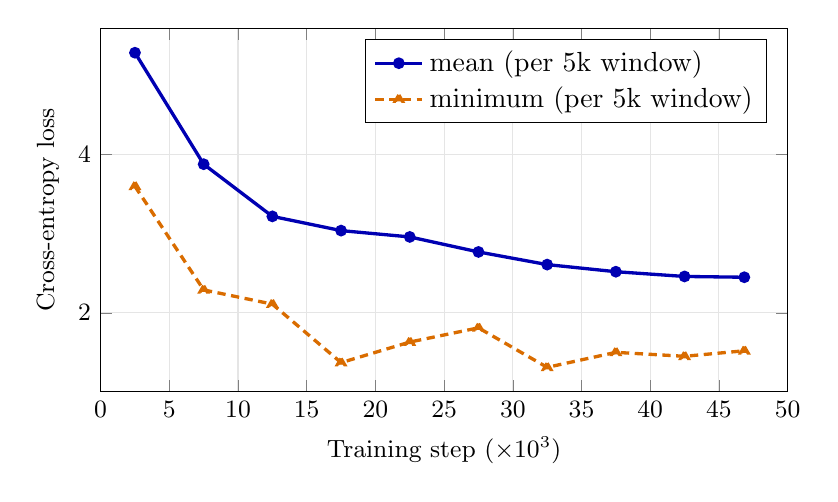
\begin{tikzpicture}
\begin{axis}[
    width=0.85\linewidth, height=6.2cm,
    xlabel={Training step ($\times 10^{3}$)},
    ylabel={Cross-entropy loss},
    xmin=0, xmax=50, ymin=1, ymax=5.6,
    grid=both, grid style={gray!20},
    legend pos=north east, legend cell align=left,
    tick label style={font=\small}, label style={font=\small},
    every axis plot/.append style={very thick},
]
\addplot[blue!70!black,mark=*,mark size=1.5pt] coordinates {
  (2.5,5.29)(7.5,3.88)(12.5,3.22)(17.5,3.04)(22.5,2.96)
  (27.5,2.77)(32.5,2.61)(37.5,2.52)(42.5,2.46)(46.85,2.45)};
\addlegendentry{mean (per 5k window)}
\addplot[orange!85!black,mark=triangle*,mark size=1.5pt,densely dashed] coordinates {
  (2.5,3.60)(7.5,2.29)(12.5,2.11)(17.5,1.37)(22.5,1.63)
  (27.5,1.81)(32.5,1.31)(37.5,1.50)(42.5,1.45)(46.85,1.52)};
\addlegendentry{minimum (per 5k window)}
\end{axis}
\end{tikzpicture}
\caption{Smoothed from-scratch training loss. The mean trends monotonically to
$\sim$2.5, resolving the prior ``loss stuck above 3.5'' failure; instantaneous
minima fall as low as 1.31.}
\label{fig:loss}
\end{figure}

\begin{table}[h]
\centering
\caption{Smoothed training loss (mean and minimum per 5000-step window).}
\label{tab:losscurve}
\small
\begin{tabular}{@{}lrr@{}}
\toprule
\textbf{Step window} & \textbf{Mean loss} & \textbf{Min loss} \\
\midrule
0 -- 4\,999       & 5.29 & 3.60 \\
5\,000 -- 9\,999  & 3.88 & 2.29 \\
10\,000 -- 14\,999 & 3.22 & 2.11 \\
15\,000 -- 19\,999 & 3.04 & 1.37 \\
20\,000 -- 24\,999 & 2.96 & 1.63 \\
25\,000 -- 29\,999 & 2.77 & 1.81 \\
30\,000 -- 34\,999 & 2.61 & 1.31 \\
35\,000 -- 39\,999 & 2.52 & 1.50 \\
40\,000 -- 44\,999 & 2.46 & 1.45 \\
45\,000 -- 47\,700 & 2.45 & 1.52 \\
\bottomrule
\end{tabular}
\end{table}

\noindent\textit{Interpretation.} The model converges monotonically. The best
saved \emph{validation} loss is 2.68; the README prose ``past 2.5'' refers to
the \emph{training}-loss trend.

\subsection{Study B — Seq2seq fine-tuning metrics}
Source: \texttt{checkpoint-5626/trainer\_state.json} for each model
(Table~\ref{tab:ft}).

\begin{table}[h]
\centering
\caption{Seq2seq fine-tuning metrics (1 epoch each).}
\label{tab:ft}
\small
\begin{tabular}{@{}lrr@{}}
\toprule
\textbf{Metric} & \textbf{DistilBART} & \textbf{FLAN-T5} \\
\midrule
Epochs                          & 1.0 & 1.0 \\
Global steps                    & 5\,626 & 5\,626 \\
Train batch size                & 8 & 8 \\
First logged train loss (step 50)  & 2.72 & 2.74 \\
Last logged train loss (step 5\,600) & 1.73 & 2.22 \\
\textbf{Eval loss (epoch 1)}    & \textbf{2.23} & \textbf{2.40} \\
Eval runtime                    & 34.2\,s & 9.7\,s \\
Eval throughput                 & 43.8 smp/s & 154.8 smp/s \\
Total FLOPs                     & $3.48\times10^{16}$ & $8.37\times10^{15}$ \\
\bottomrule
\end{tabular}
\end{table}

\noindent\textit{Interpretation.} DistilBART reaches a lower eval loss
(2.23 vs.\ 2.40), consistent with its larger capacity and summarization
pre-training; FLAN-T5-small is $\sim$3.5$\times$ faster at evaluation and
$\sim$4$\times$ cheaper in FLOPs.

\subsection{Study C — End-to-end benchmark}
Source: \texttt{evaluation/results.csv} --- 30 runs (3 models $\times$ 10 use
cases), timestamped 20 April 2026 (Table~\ref{tab:bench}).

\begin{table}[h]
\centering
\caption{End-to-end benchmark, committed run (3 cloud models).}
\label{tab:bench}
\small
\begin{tabularx}{\linewidth}{@{}l c c R R R R@{}}
\toprule
\textbf{Model} & \textbf{n} & \textbf{Succ.} & \textbf{Avg time} & \textbf{Time range} & \textbf{Avg qual.} & \textbf{Avg mem (KB)$^{\dagger}$} \\
\midrule
\texttt{qwen}    & 10 & 100\% & 66.9\,s & 7.9--122.7\,s & \textbf{0.96} & 5\,610 \\
\texttt{mistral} & 10 & 100\% & 54.8\,s & 7.4--221.5\,s & 0.80 & 324 \\
\texttt{llama4}  & 10 & 100\% & \textbf{26.6\,s} & 20.7--33.1\,s & 0.70 & 9\,378 \\
\bottomrule
\end{tabularx}
\par\vspace{2pt}
\footnotesize $^{\dagger}$\,\texttt{tracemalloc} peak Python allocations at the
agent layer --- \emph{not} model weight residency. Heavy cloud inference is
server-side, so these reflect orchestration overhead only.
\end{table}

\begin{table}[h]
\centering
\caption{Per-model quality distribution (10 use cases each).}
\label{tab:qdist}
\small
\begin{tabular}{@{}llc@{}}
\toprule
\textbf{Model} & \textbf{Quality scores (sorted)} & \textbf{\# perfect (1.0)} \\
\midrule
\texttt{qwen}    & 0.8, 0.8, 1.0, 1.0, 1.0, 1.0, 1.0, 1.0, 1.0, 1.0 & 8 / 10 \\
\texttt{mistral} & 0.4, 0.4, 0.6, 0.8, 0.8, 1.0, 1.0, 1.0, 1.0, 1.0 & 5 / 10 \\
\texttt{llama4}  & 0.4, 0.4, 0.4, 0.6, 0.6, 0.8, 0.8, 1.0, 1.0, 1.0 & 3 / 10 \\
\bottomrule
\end{tabular}
\end{table}

\begin{table}[h]
\centering
\caption{Per-category mean quality across all three models.}
\label{tab:qcat}
\small
\begin{tabular}{@{}lr@{}}
\toprule
\textbf{Category} & \textbf{Mean quality ($n=3$)} \\
\midrule
Factual          & 1.00 \\
Coding           & 1.00 \\
Technical How-To & 0.93 \\
Financial        & 0.93 \\
Comparative      & 0.80 \\
Trend Analysis   & 0.80 \\
Current Events   & 0.73 \\
Multi-hop        & 0.73 \\
Ambiguous        & 0.67 \\
Scientific       & 0.60 \\
\bottomrule
\end{tabular}
\end{table}

\noindent\textit{Interpretation.} Closed, factual, and procedural queries score
highest; \emph{Scientific}, \emph{Ambiguous}, and \emph{Multi-hop} are hardest
--- partly genuine difficulty, partly metric artefact (e.g.\ a correct
quantum-computing answer that never uses the expected keyword ``google'' is
penalised).

% =====================================================================
\section{Threats to Validity}
% =====================================================================
\begin{enumerate}\itemsep2pt
  \item \textbf{Quality metric is lexical, not semantic.} Keyword coverage
        cannot distinguish a sourced claim from a hallucinated one, nor credit a
        correct paraphrase lacking the exact keyword.
  \item \textbf{\texttt{success} $\neq$ correctness.} It only means ``no
        exception.'' Two \texttt{mistral} runs (use cases 3 and 6) returned raw
        tool-call JSON rather than prose yet were marked successful (and scored
        0.4).
  \item \textbf{Local / fine-tuned models absent from Study~C.} The committed
        benchmark covers only the three cloud models; cross-family quality
        comparison is not yet evidenced by the CSV.
  \item \textbf{Memory figures are not model footprints.} \texttt{tracemalloc}
        captures Python-level allocations only.
  \item \textbf{Validation breadth (Study~A).} Validation loss is computed over
        $\leq$100 batches every 500 steps; the single best value (2.68) is
        reported.
  \item \textbf{Single benchmark run.} No repeated trials, hence no variance or
        confidence intervals on latency or quality.
  \item \textbf{Small custom corpus.} The agent-grounded set is eight examples;
        its contribution is qualitative (format/style grounding), not
        statistical.
\end{enumerate}

% =====================================================================
\section{Reproducibility}
% =====================================================================
Key artefacts and the commands that regenerate each study are listed below
(Table~\ref{tab:artefacts}).

\begin{table}[h]
\centering
\caption{Artefacts underlying each study.}
\label{tab:artefacts}
\small
\begin{tabularx}{\linewidth}{@{}l L@{}}
\toprule
\textbf{Artefact} & \textbf{Path} \\
\midrule
From-scratch model + loop   & \texttt{training/model.py}, \texttt{training/train\_scratch.py} \\
Training log / checkpoints  & \texttt{training/checkpoints/\{training\_log.json, best.pt, latest.pt\}} \\
Seq2seq fine-tuning         & \texttt{training/finetune.py}; states in \texttt{finetuned\_*/\_checkpoints/checkpoint-5626/trainer\_state.json} \\
Dataset builder / data      & \texttt{training/create\_dataset.py}, \texttt{training/dataset.json}, \texttt{training/data\_utils.py} \\
Benchmark harness / results & \texttt{evaluation/benchmark.py}, \texttt{evaluation/use\_cases.py}, \texttt{evaluation/results.csv} \\
Model registry / config     & \texttt{configs/settings.py} \\
\bottomrule
\end{tabularx}
\end{table}

\begin{lstlisting}[language=bash]
# From-scratch training (Study A)
python training/train_scratch.py            # full run
python training/train_scratch.py --test     # smoke test

# Seq2seq fine-tuning (Study B)
python training/finetune.py --model distilbart --epochs 1
python training/finetune.py --model flan-t5   --epochs 1

# Benchmark (Study C)
python evaluation/benchmark.py
\end{lstlisting}

\noindent
\textbf{Key hyperparameters (verified from saved checkpoints).}
From-scratch: \texttt{lr=3e-4}, \texttt{wd=0.05}, \texttt{dropout=0.1},
\texttt{batch=4x8}, \texttt{warmup=2000}, \texttt{epochs=3},
\texttt{max\_seq\_len=2048}, \texttt{d\_model=768}, \texttt{n\_layers=12},
\texttt{n\_heads=12}, \texttt{d\_ff=2048}, \texttt{vocab=50257+8}.
Seq2seq: \texttt{lr=5e-5}, \texttt{batch=8}, \texttt{epochs=1},
\texttt{max\_input=512}, \texttt{max\_target=128}.

\vspace{1em}
\noindent\rule{\linewidth}{0.4pt}\\[2pt]
\footnotesize All numbers in this report were read directly from committed
artefacts (\texttt{training\_log.json}, \texttt{best.pt}/\texttt{latest.pt}, the
two \texttt{trainer\_state.json} files, and \texttt{results.csv}) on 1~June
2026.

\end{document}
